% Geometry setup
\documentclass[14pt,a4paper]{article}
\usepackage[margin=1.5cm]{geometry}

% Language setup
\usepackage[T1]{fontenc} % Output character encoding
\usepackage[utf8]{inputenc} % Input character encoding

% Spacing setup
\setlength{\parindent}{0pt} % No paragraph indenting
\setlength{\parskip}{5pt} % Set spacing between paragraphs
\frenchspacing
\newcommand{\rmspace}{\vspace{-19pt}}

% Dependency setup
\usepackage{amsmath}
\usepackage{amssymb}
\usepackage{listings}
\usepackage{float}
\usepackage{graphicx}
\usepackage{hyperref}
\usepackage{url}
\usepackage[comma,authoryear]{natbib}
\usepackage[shortlabels]{enumitem}

% Code pretty print
\usepackage{minted}

% Hyperlink format
\usepackage{xcolor}
\hypersetup{
    colorlinks,
    linkcolor={red!50!black},
    citecolor={blue!50!black},
    urlcolor={blue!80!black}
}

% Title setup
\title{Practice Session Notes: Theory of Algorithms}
\author{Viktória Nemkin (nemkin@cs.bme.hu)}
\date{}

% Custom commands
\newcommand{\lineparagraph}[1]{\paragraph{#1}\mbox{}\\}

% Document
\begin{document}
\maketitle

These are my practice session notes for the Wednesday 16:15 - 18:00 sessions, typed up into a \LaTeX{} form.

This is a work in progress, I will be updating these whenever I have time.

\textbf{Mistakes are possible}, if you spot any or if you have any questions about these notes, please contact me at nemkin@cs.bme.hu or in MS Teams.

\tableofcontents
\section{O, $\Omega$, $\Theta$, pattern matching}
\subsection{Sesssion 1, Exercise 11}

Note: this is a hard exercise, using probability theory as well, it is not included in the exam!

\lineparagraph{Exercise}

Prove that the expected running time of Simple search is $O(n)$, when both the text and pattern are random $0$ - $1$ sequences (the bits are independent of each other and probabilities of $0$ and $1$ are both $\frac{1}{2}$). What happens if only the pattern is random?

\lineparagraph{Solution}

The pattern is denoted by $M$ and its length is $m=|M|$, the text is denoted by $S$ and its length is $n=|S|$.

Let's denote with the random variable $t_i$ the number of comparisons made by the Simple search algorithm for a pattern position with a shift of $i$ number of characters.

Then, in total the number of comparisons made is $\sum\limits_{i=0}^{n-m}t_i$, so the expected number of comparisons is $E(\sum\limits_{i=0}^{n-m}t_i)$.

$E(\sum\limits_{i=0}^{n-m}t_i) = \sum\limits_{i=0}^{n-m}E(t_i)$, due to the Linearity of Expectation. It is important to remember, that this holds true even when the variables are correlated, like in our case!

Now, the only thing left to find is $E(t_i)$.

For a given position $k$ in the pattern, the probability of it matching the current position in the text, or $P(S[k+i] = M[k])$ is $\frac{1}{2}$, since both the pattern and the text is random, and they match for $S[k+i] = M[k] = 0$ and $S[k+i] = M[k] = 1$ while not match for $S[k+i] = 0, M[k] = 1$ and $S[k+i] = 1, M[k] = 0$, all four of these happen with $\frac{1}{4}$ probability, and two of these are the desired.

Now, the comparisons are made up until the point one of them fails, and we care about the number of them. This would be a geometric distribution, if the number of possible positions would be infinite. While this is not true, since the pattern and the text are both finite, since we only care about an upper bound, we can over-estimate the expectation value with the geometric distribution's expectation value.

$E(t_i) \leq{} \sum\limits_{j=1}^{\infty}j2^{-j} = 2$.

Then we plug this back in:

$E(\sum\limits_{i=0}^{n-m}t_i) = \sum\limits_{i=0}^{n-m}E(t_i) \leq{} \sum\limits_{i=0}^{n-m}2 = 2(n-m+1) \in{} O(n)$.

When only the pattern is random, the only thing changing here is how we calculate $P(S[k+i] = M[k])$. If the text's character is a $0$, or $S[k+i]=0$ then the probability of a random $M[k]$ matching it is $\frac{1}{2}$, when $M[k]=0$. Similarly, if the text's character is a $1$, or $S[k+i]=1$ then the probability of a random $M[k]$ matching it is $\frac{1}{2}$, when $M[k]=1$. So the probability is the same and the same result holds here as well.\pagebreak
\subsection{Session 1, Exercise 12}

Note: this is a hard exercise, it is not included in the exam!

\lineparagraph{Exercise}

Algorithm A solves the problem of pattern matching for $0$ - $1$ sequences, in case of pattern of $m$ bits and text of $n$ bits it uses $T(n, m)$ steps to give all occurrences of the pattern (in increasing order). How can this be used to find all occurrences of a length $m$ pattern in a length $n$ text over an arbitrary alphabet $\Sigma$ using $O((n + T(n, m))log_2|\Sigma|)$ time?

\lineparagraph{Solution}

Let's just say that $O((n + T(n, m))log_2|\Sigma|)$ is suspiciously specific. Especially the $log_2|\Sigma|$ part indicates that we should encode the alphabet in binary form, then a length of an original character in binary will be $log_2|\Sigma|$ in this new alphabet.

However, an issue with this approach will be, that only whole-character shifts should be allowed. We can not allow the algorithm to shift the pattern by half a binary-encoded character's length and find a match there. There is another issue, where this would also result in $T(log_2|\Sigma|n, log_2|\Sigma|m)$ runtime for $A$ and we have no idea about the inner workings of $T$ to somehow estimate this using $T(n,m)$.

Both of these issues will be solved, if we instead create $k = \lceil log_2|\Sigma| \rceil$ number of different pattern matching tasks, and the $i$th task will contain the original task's characters replaced by their $i$th bits.

Now if we let the algorithm find all the occurrences, if it finds let's say an occurrence with shift $a$ in all of the $k$ tasks, that means that all of the bits of the characters match, so the original pattern matches the original text with shift $a$ as well!

To keep track of the results of the $k$ tasks, we create an array $Z$ of length $n$, initialized with $0$'s at the beginning. If the algorithm on the $i$th task finds an occurrence with shift $a$, it increments $Z[a]$ with $1$. Then, at the end when all algorithms finished we read $Z$ and if the value at position $a$ is $k$ that means that all of the $k$ tasks found that as a match, so the original pattern matches with shift $a$ as well.

Finally, the number of steps required to run $A$ on $k$ tasks with the same length as the original string but in binary is $kT(n, m)$, while initializing and incrementing the $Z$ array (of size $n$) is at most $nk$, so in total we are at $O((n+T(n,m))k)$ steps, which is $O((n+T(n,m))log_2|\Sigma|)$.
\pagebreak
\section{Finite Automata}
\subsection{Session 2, Exercise 7}

\lineparagraph{Exercise}

Give a nondeterministic finite automaton that accepts those words that have 10100 as subword.

\lineparagraph{Solution}

The key to solving this exercise using a nondetermnistic automaton is to create a delayed start on the starting state by introducing a 0,1 loop on it:

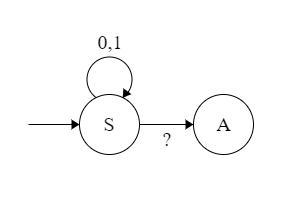
\includegraphics[width=200px]{02/wait_to_start.png}

This will "eat up" some prefix of the input word before allowing the computation to proceed to state A. Whatever we put in place of the ? on the leaving transition will be a nondeterministic choice for the automaton.

The next step is to add the success path to the automaton which contains the string we want to have as a subword: 10100.

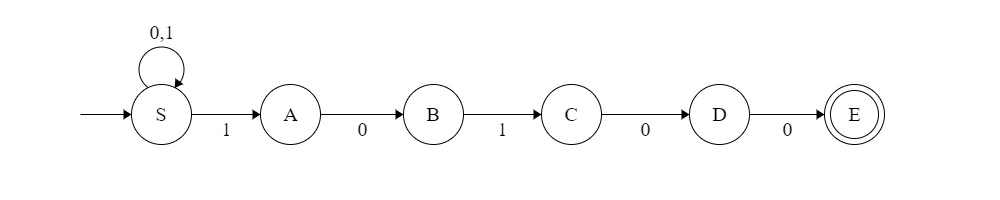
\includegraphics[width=\linewidth]{02/success_path.png}

Then finally, let's allow "eating up" any remaining suffix of the word as well:

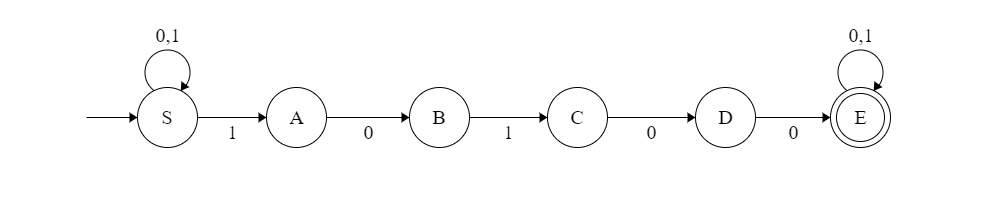
\includegraphics[width=\linewidth]{02/10100.png}

Some observations:

\begin{itemize}
    \item Firstly, this is a nondeterministic finite automaton: Notice how in state $S$, for an input character of $1$ we can either remain in $S$, or move to state $A$.
    \item There are also transitions missing: it is an incomplete finite automaton as well. For example, in state $A$, for an input character of 1, the machine halts (and halting due to a missing transition means rejection, \textbf{regardless of the current state's accept/reject status}.
    \item Notice how visually similar this automaton is to the regular expression for the same language: $(0+1)^*10100(0+1)^*$.
\end{itemize}

Let's look at an example computation on the word 1110100, which is in the language of the automaton.

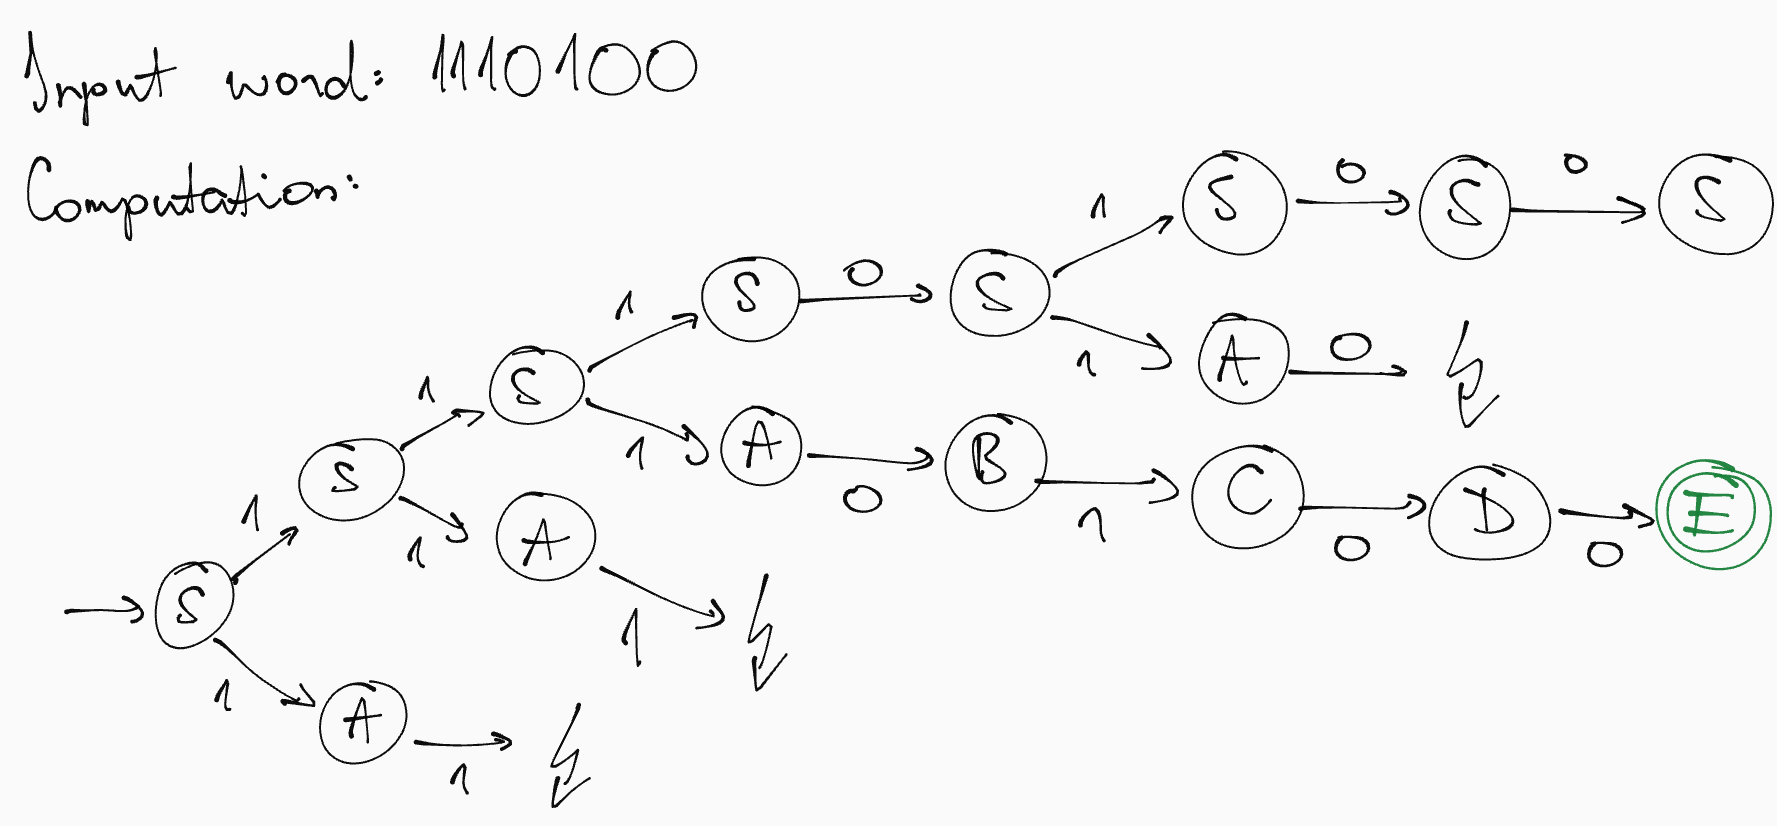
\includegraphics[width=\linewidth]{02/computation_1110100.png}

\begin{itemize}
    \item See, how it tried to leave state $S$ and move to state $A$ many times in different places of the input string? Many times it failed, when the timing was incorrect. Maybe it was too early, when the first two 1's, which are not part of the matching subword were given to it, or it was too late, when the pattern was already gone.
    \item There was already a lazy case, the top branch, which just remained in state $S$ forever, which also could not succeed.
    \item However there only needs to be a single successful branch and it only needs to time its move to state $A$ correctly once: on the third branch it successfully finished in state $E$, which means that the word is accepted, correctly!
    \item Notice how it is only possible to reach state $E$, when the input word contains 10100. We need a 1 to move from $S$ to $A$, then we need a consecutive $0$ to move from $A$ to $B$, then we need a consecutive $1$ to move from $B$ to $C$, then we need a consecutive $0$ to move from $C$ to $D$, then we need another consecutive $0$, to move from $D$ to $E$.
    \item When the timing is just right and we catch the beginning of the pattern we can ''sail smoothly'' towards $E$.
\end{itemize}

When you are on the exam, you will need to give some sort of proof that the automaton you wrote up does what the exercise is asking you to do. For this exercise this is how a proof like this might look like:

\textbf{Proof:}

1. Let's look at the states of the automaton:
What the different states mean and why their transitions are correct.
\begin{itemize}
    \item State $S$ is the starting state. Here, we non-deterministically wait to start our computation, using the $0$,$1$ loop. Since the first character of the pattern we seek is a $1$, on an input character of $1$, the automaton can decide to move to state $A$.
    \item State $A$ represents the information "already read the first character of the pattern". Here, we allow a transition to state $B$ if the second character of the pattern comes, which is a $0$. However, the transition for an input of $1$ is missing, which means that the computation (on that branch) will halt. This is correct, because the pattern's characters must be consecutive.
    \item States $B$, $C$ and $D$ work similaly: they represent the next character recognized from the pattern we seek and we only allow a transition for the upcoming character from the pattern to move forward, towards $E$.
    \item Finally, state $E$ represents "pattern found". This means that we can accept the word, furthermore, any further input characters are allowed, since the pattern can be anywhere in the word.
\end{itemize}

2. Let's look at the accepted and rejected words of the automaton:

Any word that contains the pattern 10100 will be accepted, because the automaton on the (single) accepting branch of the computation first non-deterministically reads the prefix of the word before the pattern, then transitions from $S$, to $E$ using the consecutive characters of the pattern, then finally in state $E$ further characters can be read (the remaining suffix of the word) and the word will be accepted.

Any word that does not contain the pattern 10100 can not reach state $E$, because each step towards $E$ requires the next character of the pattern to be present consecutively in the word. There is correct timing to leave $S$, no computational branch can end up in $E$, so the word will be rejected.

\textbf{(End of proof.)}

(Due to time limits on the exam, it is okay to not use full sentences like I did above, abbreviate things, etc.)

It is important when doing these proofs, that you do not use a specific input word as an example, but generalize to any possible words, like the proof above.

\lineparagraph{Deterministic solution}

This exercise allows us to truly appreciate nondeterministic automata, since it made it really easy for us to come up with a design for a given subword.

However, the task is also possible with a deterministic automaton (it must be, since we can convert any NFA into a DFA, but there is an even easier method to obtain a DFA, than the general conversion algorithm). This is not part of the task, but nice to see how it works as well.

Step 1: Get rid of loop on the starting state, we need to be deterministic now.

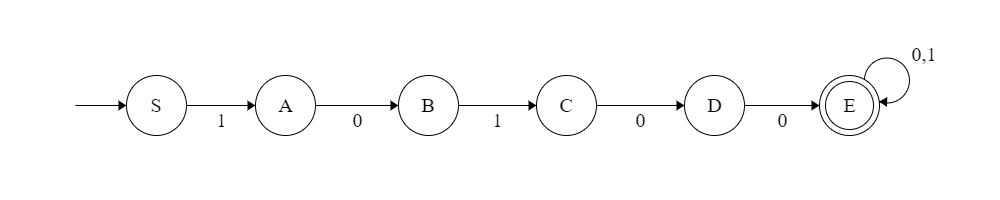
\includegraphics[width=\linewidth]{02/det_10100_1.png}

Step 2: Put in the missing transitions, states $S$-$D$ all miss 1 of them.

The main idea here is that the missing transitions are failures in recognizing the next character of the pattern at the current position. How big of a failure it is depends on what the pattern we have found so far is and how much of it can be salvaged when we add the incorrect character at the end.

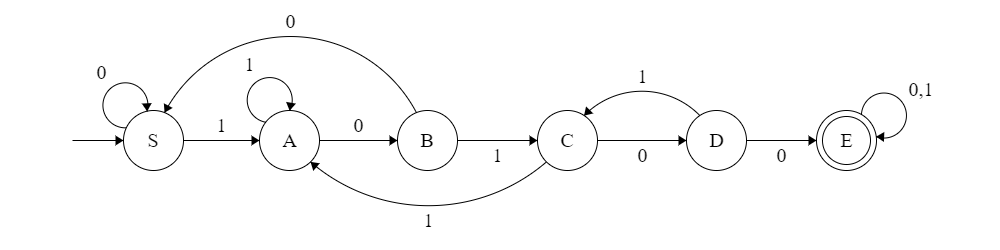
\includegraphics[width=\linewidth]{02/det_10100_2.png}

\begin{itemize}
    \item When we are in state $S$, the pattern we have found so far is nothing. Until we read $0$'s we remain in state $S$, since the first character of the pattern is a $1$.
    \item When we are in state $A$, the pattern we have found so far is ''$1$''. If we read another $1$ now, we now have ''$11$''. The pattern is ''$10100$'', so that second $1$ character can still turn out to be the beginning of the pattern, so we need to remember that we have a ''$1$'' and thus stay in state $A$.
    \item When we are in state $B$, the pattern we have found so far is ''$10$'', if we read a $0$ in now, that makes it a ''$100$''. Unfortunately, there is no salvaging this: not ''$100$'', not ''$00$'' and not even a single ''$0$'' is useful for us, neither of them are the prefixes of the pattern ''$10100$''. We need to scratch everything and go back to state $S$.
    \item When we are in state $C$, the pattern we have found so far is ''$101$''. If we read a $1$ now, that makes it ''$1011$''. The possible suffixes to remember here are ''$011$'', ''$11$'' and ''$1$''. In general we always need to keep the longest one that is still a prefix of the pattern: in this case, that is ''$1$'', which is represented by state $A$, so we move back there.
    \item When we are in state $D$, the pattern we have found so far is ''$1010$''. If we read a $1$ now, that makes it ''$10101$''. This is great news, because we can actually just forget the first two characters and we can still keep the remaining ''$101$'', which is the first three characters of the pattern! Not much is lost, ''$101$'' is represented by state $C$, so we can move there.
\end{itemize}\pagebreak
\subsection{Session 2, Exercise 10}

\lineparagraph{Exercise}

Let $\Sigma = \{0, 1\}$. The sequences are considered as binary numbers. Give a finite automaton that accepts exactly those words that represent numbers divisible by three in binary form. Take into consideration that a number does not begin with $0$, except for number zero itself, and that the input number is read beginning with the most significant digit.

\lineparagraph{Solution}

Any automaton that we design will work by reading the input binary string from left to right. We will want to keep track of the remainder of the current binary number after each 0 or 1 we read. The question is how do we update this remainder when the next input character comes? First, let's do a simpler task, just keeping track of the number itself and updating it as we go.

\begin{itemize}
    \item For example, let's say that so far we have read the the ''$101$'' binary string on the input. That is a $5$ in decimal form.
    \item Let's say the next character is also a $1$, so now the current string is ''$1011$'', or in decimal form $11$.
    \item This was achieved by shifting the string ''$101$'' to the left and adding a ''$1$'' as the least significant character.
    \item A left shift in binary corresponds to multiplication by $2$ in decimal, and then if the next character is a $1$, we just need to add $1$ to the decimal value as well. So in our example, $5*2 + 1 = 11$.
    \item In general, if we read a binary number from left to right, to calculate its decimal value, we simply multiply the current decimal value by $2$, and if the bit we read was a $1$, we add a $1$ and continue to the next bit.
\end{itemize}
 
If we don't care about the entire number, just its remainder when divided by $3$, we can do the same calculation, but modulo $3$.

If the current number is divisible by $3$, or in the form $3k$, and the next binary character is a $0$, then to update we do $3k*2+0 = 6k$, which means that the updated number will still be divisible by $3$.

If the next binary character is a $1$, then to update we do $3k*2+1=6k+1=3*(2k)+1$, which means that the updated number has a remainder of $1$ when divided by $3$.

We can represent these statements by the following two transitions from state $3k$:

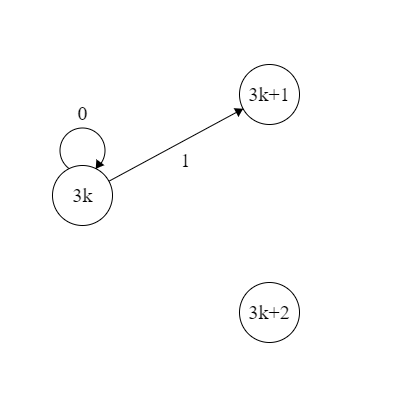
\includegraphics[width=250px]{02/modulo_1.png}

If the current number has a remainder of $1$, when divided by $3$, or in the form of $3k+1$, and the next binary character is a $0$, then to update we do $(3k+1)*2+0=6k+2=3*(2k)+2$, which means that the updated number has a remainder of $2$, when divided by $3$.

If the next binary character is a $1$, then to update we do $(3k+1)*2+1=6k+3=3*(2k+1)$, which means that the updated number is divisible by $3$.

We can represent these statements by the additional two transitions from state $3k+1$:

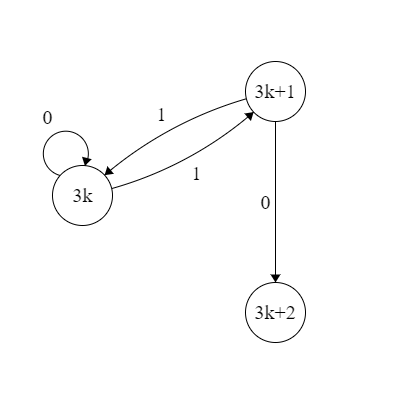
\includegraphics[width=250px]{02/modulo_2.png}

Finally, if the current number has a remainder of $2$, when divided by $3$, or in the for of $3k+2$, and the next binary character is a $0$, then to update we do $(3k+2)*2+0=6k+4=3*(2k+1)+1$, which means that the updated number has a remainder of $1$, when divided by $3$.

If the next binary character is a $1$, then to update we do $(3k+2)*2+1=6k+5=3*(2k+1)+2$, which means that the updated number has a remainder of $2$, when divided by $3$.

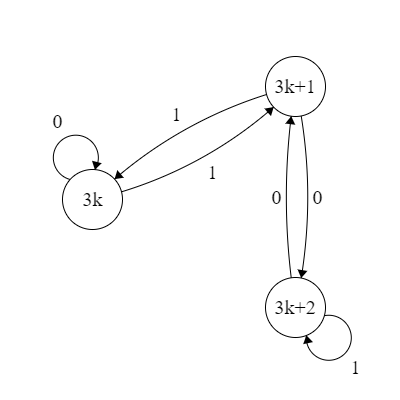
\includegraphics[width=250px]{02/modulo_3.png}

If you want to try this automaton, come up with any decimal number, turn it into binary form and calculate its remainder by $3$, by applying the transitions above using its binary form as input. The starting state should be $3k$, since when we have not read anything in yet, so we want to start from a state that is equivalent to the number $0$, which is divisible by $3$.

I however, did not mark a starting state yet on this image, because there is one additional statement to keep in mind: ''Take into consideration that
a number does not begin with $0$, except for number zero itself.''. This means that we do not consider any string longer than 1 characters starting with a $0$ a number, much less a number that is divisible by $3$, so we need to reject these words.

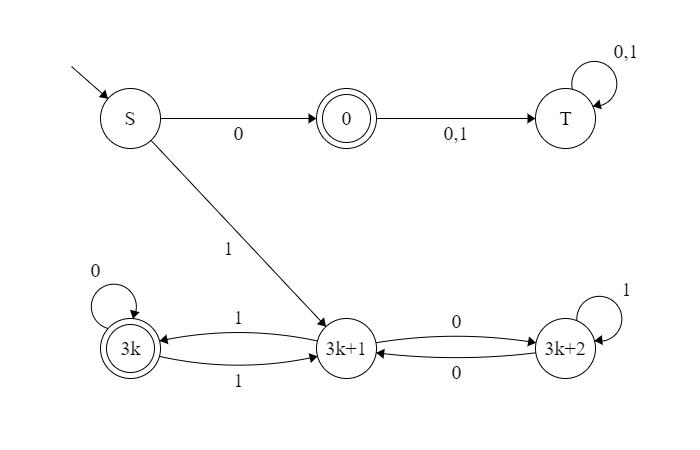
\includegraphics[width=\linewidth]{02/modulo_final.png}

Now, if this was an exam, here is how to prove that this accepts the language: (Basically everything I just said, but in a shortened form.)

\textbf{Proof:}

1. Let's explain what the different states mean and that their transitions are correct:

\begin{itemize}
    \item $S$ is the starting state. If we read a $0$ in, we move to a state dedicated to the number $0$. If we read a $1$ in, we move to the state that represents binary numbers, that give a remainder of $1$ when divided by $3$, which is true for the (binary) number $1$.
    \item The only word for state $0$ is $0$ itself, this is divisible by $3$ and is accepted. If we read anything else after a $0$ that is an incorrectly formatted number and moves to a trap state $T$ which rejects it.
    \item The states $3k$, $3k+1$ and $3k+2$ represent the 3 remainder classes of division by $3$. When a new character is read on the input, we update the remainder class with multiplying by $2$ (binary shift) and adding the $0$ or $1$ bit we just read. We can see that the transitions are correct, since:
    \begin{itemize}
        \item $3k*2+0 = 3*(2k)$
        \item $3k*2+1 = 3*(2k)+1$
        \item $(3k+1)*2+0 = 3*(2k)+2$
        \item $(3k+1)*2+1 = 3*(2k+1)$
        \item $(3k+2)*2+0 = 3*(2k+1)+1$
        \item $(3k+2)*2+1 = 3*(2k+1)+2$
    \end{itemize}
\end{itemize}

2. Let's explain that the correct words are accepted and the words not in the language are rejected:

The words in the language are any numbers that are divisible by $3$, which is either the number $0$ or anything that is in the form $3k$, these states are accepting.

A word could be outside of the language due to being malformed (starting with $0$, but not being $0$ itself), which will be redirected to a trap $T$; or due to not being divisible by $3$, in which case it will land in either $3k+1$ or $3k+2$ and will be rejected there. Finally, the empty string is rejected because it's not a number, which is the only word that will end up in state $S$.

\textbf{(End of proof.)}

Notes:

\begin{itemize}
    \item I ended up making a deterministic automaton here, however the task would allow a non-deterministic one as well. We could get rid of the enitre $T$ state and define no transitions outwards from state $0$. If there is input left to be read in state $0$ the automaton halts due to a missing transition, which rejects the word regardless of the accept/reject status of the current state!
\end{itemize}\pagebreak
\section{Regular expressions, context-free languages}
\subsection{}
\label{3.1}

\lineparagraph{Exercise}

Let $\Sigma = \{a,b\}$ and let language $L$ consist of words
that contain the same number of $a$'s and $b$'s. Is $L$ regular?

\lineparagraph{Solution}

\textbf{Gut feeling} (This is not yet a proof!)

Not regular.

This language is similar to $a^nb^n$ (studied in the lecture). The
main issue with it will be similar: we would need to remember the difference
of the number of $a$'s and $b$'s we have read in so far and only
accept the word if the difference is $0$ after reading in the entire
word.

For every possible difference, we will need a separate state, however the
difference can be arbitrarily large, while we can only have a finite
number of states using Finite Automata, so it won't be possible
to construct such a machine.

\textbf{Proof}

We will do proof by contradiction:

\begin{itemize}
    \item Let's assume that $L$ is regular.
    \item Then, that means that there exists a Deterministic Finite Automata, that accepts the language $L$.
    \item Let's take one such automata, and name it $M$.
    \item Let's count the number of states in $M$ and name this number $n$.
    \item Now let's list exactly $n+1$ specifically chosen words from the $L$ language: $ab$, $aabb$, $a^3b^3$, $\dots$, $a^{n+1}b^{n+1}$.
    \item Then imagine feeding these $n+1$ words into $M$. For all of them, let $M$ read in the $a$ letters and then stop and take note of which state the word is at the moment, halfway-through the operation.
    \item After reading in $a$, $aa$, $a^3$, $\dots$, $a^{n+1}$, since these are $n+1$ cases, while $M$ only has $n$ states, we can use the \href{https://en.wikipedia.org/wiki/Pigeonhole_principle}{Pigeonhole Principle} and say, that there exists at least two different half-words $a^i$ and $a^j$ $(i\neq{}j)$, for which $M$ arrived at the same state after feeding it these inputs. Let's name this state $S$.
    \item Since $a^ib^i$ is in language $L$, it must be accepted by $M$. This means that when we continue from state $S$ and feed in the $b$'s of the word, the machine must arrive in an accepting state. So there exists a path from state $S$ to an accepting state that is traversed by the input $b^i$.
    \item However, $M$ also arrives in state $S$ when it reads $a^j$. We just noted, that if from $S$ it reads $b^i$ it will arrive in an accept state. If we put these two together, it means that $M$ accepts the word $a^ib^j$, where $i\neq{}j$, which is \textbf{not} in $L$, since it doesn't have the same number of $a$'s and $b$'s.
    \item We stated in the beginning that $M$ is a machine whose language is $L$, however we just found a word that is not in $L$, but accepted by $M$, so this is a contradiction.
\end{itemize}

Notes:

\begin{itemize}
    \item This is symmetric, we could also prove that $M$ accepts $a^ib^j$, for $i\neq{}j$ which is also a contradiction, since that word is also not in $L$.
    \item To put it shortly: the machine cannot distinguish $a^i$ and $a^j$ $(i\neq{}j)$ and since $a^ib^i$ and $a^jb^j$ are accepted, so are $a^ib^j$ and $a^jb^i$, which are not in $L$, which is a contradiction.
    \item Note, that this proof is exactly the same as the proof for language $a^nb^n$ studied in the lecture. This is due to the fact, that these languages are similar, for both of them the issue is keeping track of the number of $a$'s to (eventually or simultaneously) compare them to the number of $b$'s.
    \item It is \textbf{not true}, that ''the proof works because $a^nb^n$ is a subset of $L$''. For example, $a^nb^n$ is also a subset of $\Sigma^*$, which is regular!
\end{itemize}
\pagebreak
\subsection{Session 3, Exercise 2}

\lineparagraph{Exercise}

Let $\Sigma = \{(,)\}$. Prove that the language of properly matched parentheses sequences is not regular.

\lineparagraph{Solution}

Quite similar to \ref{3f1}. The $n+1$ words from $L$, the language of properly matched parentheses to be used are $()$, $(())$, $(^3)^3$, $\dots$, $(^{(n+1)})^{(n+1)}$, so just substitute $a = ($ and $b = )$.\pagebreak
\subsection{Session 3, Exercise 3}

\lineparagraph{Exercise}

Is the language regular, that consists of sequences of $0$'s of a length that is...
\begin{enumerate}[a.)]
\item an even number?
\item an odd number?
\item a perfect square?
\item a power of $2$?
\end{enumerate}

\lineparagraph{Solution}

\subsubsection{Even number of $0$'s}

Regular.

\textbf{Proof 1}: The regular expression $(00)^*$ matches them.

Proof that this regular expression matches the language:

\begin{itemize}
    \item The $^*$ operator allows any number of repeats, even 0.
    \item Inside the $^*$ operator we have two $0$'s, which can be repeated any number of times to match any even number of $0$'s.
    \item The empty string, also known as zero number of $0$'s contains an even number of $0$'s, so it is part of the language. $(00)^*$ matches the empty string, which is correct.
\end{itemize}

\textbf{Proof 2}: The following DFA accepts the language:

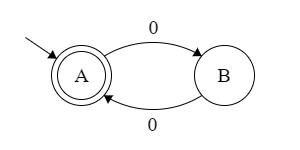
\includegraphics[width=150px]{03/even_zeroes.png}

Proof that this automaton accepts the language:

\begin{itemize}
    \item Words that end up in state $A$ are the words that contain an even number of $0$'s, while words that end up in state $B$ contain an odd number of $0$'s.
    \item The empty string is correctly accepted.
    \item From state $A$, reading another $0$ moves to state $B$, so after reading an even number of $0$'s, if we read one more, now we have an odd number of $0$'s.
    \item And similarly for state $B$.
\end{itemize}

\subsubsection{Odd number of $0$'s}

Regular.

\textbf{Proof 1}: The regular expression $0(00)^*$ matches them.

Proof that this regular expression matches the language:

\begin{itemize}
    \item We have just seen that $(00)^*$ matches an even number of $0$'s.
    \item Adding the $0$ at the front will then match an odd number of $0$'s.
\end{itemize}

\textbf{Proof 2}: The following DFA accepts the language:

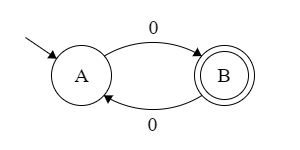
\includegraphics[width=150px]{03/odd_zeroes.png}

Proof that this automaton accepts the language:

\begin{itemize}
    \item This is the same automaton as in the previous exercise, but now the accept state is $B$, to accept an odd number of $0$'s.
\end{itemize}

\subsubsection{A perfect square number of $0$'s}

\textbf{Gut feeling} (This is not yet proof!)

Not regular.

The issue here is going to be, that the length of the accepted words get further and further away from each other as the length of the words increases. We always need to keep track of how far away we are from the next accepted word, how many more $0$'s we need to finally accept. We would need separate states for each of these "$x$ number of $0$'s before we can accept", however $x$ could be arbitrarily large and we only have a finite number of states.

\textbf{Proof}

 Quite similar to \ref{3.1}, the $n+1$ words to use here are of the length of the first $n+1$ square numbers: $0 = 0^{1^2}$, $0000 = 0^{2^2}$, $0^9 = 0^{3^2}$, $0^{16} = 0^{4^2}$, $0^{5^2}$, $0^{6^2}$, $\dots$, $0^{(n+1)^2}$.
 
Then, the finishing of \ref{3.1} is a bit different:

When we find that for an $i\neq{}j$, both $0^{i^2}$ and $0^{j^2}$ end up in the same state $S$, the reasoning is a bit different. Without loss of generality, we can assume that $i<j$. If we were to continue $0^{i^2}$ from state $S$ with $2i+1$ more $0$'s, then the whole input would be $0^{i^2+2i+1} = 0^{(i+1)^2}$, which means that we should accept this word, so from state $S$, for $2i+1$ number of $0$'s we must reach an accept state.

However, this also means that when we continue $0^{j^2}$ (which remember, also arrives in $S$) with $2i+1$ $0$'s, so the word is $0^{j^2+2i+1}$, we will also arrive at the same accept state.

However $j^2+2i+1$ is not a square number. It is between two consecutive square numbers $j^2$ and $(j+1)^2 = j^2+2j+1$, but not equal to either of them:
\begin{itemize}
    \item $j^2 < j^2 + 2i + 1$, since $0<i$.
    \item $j^2 + 2i + 1 < j^2 + 2j + 1$, since $i<j$.
\end{itemize}

Thus, we found a word accepted by $M$, however not in $L$, which is a contradiction.

\subsubsection{A power of $2$}

\textbf{Gut feeling} (This is not yet proof!)

Not regular, the situation is even worse than for square numbers, since powers of $2$ are even further spaced apart as the exponent continues to grow.

\textbf{Proof}

The $n+1$ words to be used are $0^{2^1}$, $0^{2^2}$, $0^{2^3}$, $\dots$, $0^{2^{n+1}}$.

Then similarly to the previous proof, when for $i\neq{}j$, $0^{2^i}$ and $0^{2^j}$ end up in the same state $S$, if we continue by $2^i$ more $0$'s, we should accept, since $0^{2\cdot{}2^i}$ is also a power of two number of $0$'s, however this means  $0^{(2^i + 2^i)}$ will also be accepted, but $2^i + 2^j$ is not a power of $2$, since $i\neq{}j$.\pagebreak
\subsection{Session 3, Exercise 4}

\lineparagraph{Exercise}

Let $\Sigma=\{0,1\}$. Determine the languages of the following regular expressions.

\begin{enumerate}[a.)]
\item $(0+1)^*011(0+1)^*$
\item $1(0+1)^*0$
\item $((0+1)(0+1))^*$
\end{enumerate}

\lineparagraph{Solution}

$(0+1)^*$ is a regular expression that accepts any string from $\Sigma^*$, since $0+1$ accepts either a $0$ or a $1$, and the $^*$ operator allows any number of repeats, including zero.

Thus, $(0+1)^*011(0+1)^*$ is a regular expression that accepts strings that can begin anyhow (including the empty string), then contain the word $011$, then end anyhow, including the empty string. Or, simply put, it accepts all words that contain the string $011$.

For $1(0+1)^*0$, the string must begin with a $1$ and must end with a $0$, while anything, including the empty string can be in between. So this regular expression accepts words that begin with a $1$ and end with a $0$.

For $((0+1)(0+1))^*$, the inner regular expression $(0+1)(0+1)$ accepts any strings with a length of two. Using the $^*$ operator on this allows this to repeat any number of times, allowing for any even length to be accepted, including the length of $0$, which is the empty string.\pagebreak
\subsection{Session 3, Exercise 5}

\lineparagraph{Exercise}

Give regular expressions for the languages over alphabet $\{0,1\}$ that consist of the following words.

\begin{enumerate}[(a)]
\item Words of odd lengths.
\item Words of even length that start and end with $1$.
\item Words containing at least three $0$'s.
\item Words containing an even number of $0$'s.
\item Words of odd lengths starting with $0$ and words of even length starting with $1$.
\item Words of odd length containing subword $00$.
\end{enumerate}

\lineparagraph{Solution}

\subsubsection{Words of odd lengths}

From the previous exercise we know, that $((0+1)(0+1))^*$ accepts the words of even lengths. If we add a $(0+1)$ at the beginning it will add one more character to the lengths, making them odd: $(0+1)((0+1)(0+1))^*$.

\subsubsection{Words of even length that start and end with 1}

To start and end with $1$'s, the regular expression will be $1\text{<something here>}1$. For <something here>, we need to add a regular expression, that together with the two other $1$'s will allow for an even number of characters. So without the two $1$'s, we need an even number of characters, for which we know the regular expression: $((0+1)(0+1))^*$. Putting these together we arrive at $1((0+1)(0+1))^*1$. Since $((0+1)(0+1))^*$ accepts the empty string, the final regular expression will also accept $11$, which is the shortest possible string in the language.

\subsubsection{Words of odd length that start and end with 1}

This was not in the exercise, however I would like to illustrate a point here.

Let's follow the same pattern of thought, as in the previous exercise:
\begin{itemize}
    \item To start and end with $1$'s, the regular expression will be $1\text{<something here>}1$. \item For <something here>, we need to add a regular expression, that together with the two other $1$'s will allow for an odd number of characters.
    \item So without the two $1$'s, we need an odd number of characters, for which we know the regular expression: $(0+1)((0+1)(0+1))^*$.
    \item Putting these together we arrive at $1(0+1)((0+1)(0+1))^*1$.
    \item We have made a mistake...
\end{itemize}

What is the shortest word in this language? It's $1$, which is not accepted by the regular expression above. The issue is that we did not think about the fact, that both starting and ending in a $1$ can also literally mean the same $1$ character, nothing more.

In general, it is always important when building regular expressions from multiple parts, to check for short strings in the language, to see if our expression works for the simplest cases as well.

In this example, to fix the regular expression above, we simply append the missing case at the end: $1(0+1)((0+1)(0+1))^*1 + 1$. This accepts words of length $1$, $3$, and so on, which is what we've wanted.

\subsubsection{Words containing at least three 0's}

Anything can go between the $0$'s, so simply $(0+1)^*0(0+1)^*0(0+1)^*0(0+1)^*$. The three $0$'s between the $(0+1)^*$'s enforce that the string must contain at least three $0$'s.

\subsubsection{Words containing an even number of 0's}

Let's start by words containing exactly two $0$'s: $1^*01^*01^*$. Then, to allow an even number of $0$'s, we can use the $^*$ operator on this: $(1^*01^*01^*)^*$. However, this regular expression has one problem: if the number of $0$'s is zero, we are unable to match anything other than the empty string. However, we would like to match $1^*$, so we can fix this, by either simply appending it at the end: $(1^*01^*01^*)^* + 1^*$, or to make it shorter, simply moving the first one outside of the outer $^*$ operator: $1^*(01^*01^*)^*$.

\subsubsection{Words of odd lengths starting with 0 and words of even length starting with 1}

Let's make two regular expressions and combine them with a $+$ at the end.

Words of odd lengths starting with $0$: $0((0+1)(0+1))^*$. $0$ matching literal $0$ at the beginning, then $((0+1)(0+1))^*$, matching the remaining even number of any characters, which in total result in an odd number of characters.

Words of even length starting with $1$: $1(0+1)((0+1)(0+1))^*$. Since the word must start with a $1$, this no longer can be an empty string. The shortest possible words are $10$ and $11$, which are correctly matched, and can be followed by an even number of characters.

Finally, combinging the two: $0((0+1)(0+1))^* + 1(0+1)((0+1)(0+1))^*$, or to make it shorter: $(0 + 1(0+1))((0+1)(0+1))^*$.

\subsubsection{Words of odd length containing subword 00}

$00$ is even length, so it either starts with an odd length string, then $00$, then an even length string or vice versa: $((0+1)(0+1))^*(0+1)00((0+1)(0+1))^* + ((0+1)(0+1))^*00(0+1)((0+1)(0+1))^*$ and we can shorten this a little like this: $((0+1)(0+1))^*((0+1)00+00(0+1))((0+1)(0+1))^*$. Again, paying attention to the shortest words in the language, which are of length three, this one can match those as well.

\pagebreak
\subsection{}

Give regular expressions that are shorter than the following ones but give the same languages.

\begin{enumerate}[a.)]
\item $(0+\varepsilon)^*$
\item $((0+\varepsilon)(0+\varepsilon))^*$
\item $(0+1)^*01(0+1)^*+1^*0^*$
\end{enumerate}\pagebreak
\subsection{}

Give a regular expression whose language consists of all words over $\{0,1\}$ without the subword 110.\pagebreak
\subsection{Session 3, Exercise 8}

\lineparagraph{Exercise}

What language is generated by the following grammar?

\begin{align*}
S &\rightarrow A | B\\
A &\rightarrow 0A1 | 01\\
B &\rightarrow 1B0 | 10
\end{align*}

\lineparagraph{Solution}

We make a decision at $S$, whether to continue with variable $A$, or $B$.

$A$ generates with the following producion rule: $A \rightarrow 0A1|01$, which will put the same number of $0$'s at the beginning as the number of $1$'s at the end, using the ''one to the left and one to the right'' method: every single activation of the $A \rightarrow 0A1$ puts one $0$ to the left and one $1$ to the right, making sure their numbers remain equal as we generate the string.

The empty string is not generated, because there is no production rule that would allow $A$ to terminate in a $\varepsilon$. This is the same as $0^n1^n$, where $n>0$: $L_A=\{0^n1^n|n>0\}$.

With similar logic, $L_B=\{1^n0^n|n>0\}$.

And finally, then $L = L_A \cup L_B$.\pagebreak
\subsection{Session 3, Exercise 9}

\lineparagraph{Exercise}

Give CF-grammars for the following regular languages from Exercise 4:

Let $\Sigma=\{0,1\}$.

\begin{enumerate}[a.)]
\item Contains $011$ as a substring: $(0+1)^*011(0+1)^*$
\item Starts with $1$, ends with $0$: $1(0+1)^*0$
\item Is of even length: $((0+1)(0+1))^*$
\end{enumerate}

\lineparagraph{Solutions}

\subsubsection{Contains $011$ as a substring}

Let's make a variable for producting $(0+1)^*$:

\begin{align*}
A &\rightarrow 0A|1A|\varepsilon
\end{align*}

$A$ generates any string from left-to right, using the first rule if the next character is a $0$ and the second rule if the next character is a $1$. When we reach the end of the string, with no more characters left, the third rule is applied and the production is completed.

Using $A$, we can now do

\begin{align*}
S &\rightarrow A011A\\
A &\rightarrow 0A|1A|\varepsilon
\end{align*}

where $S$ creates the required $011$ substring and puts an $A$ at the beginning and at the end $A$ to generate any optional characters.

\subsubsection{Starts with $1$, ends with $0$}

Using the same $A$, and the same logic as before:

\begin{align*}
S &\rightarrow 1A0\\
A &\rightarrow 0A|1A|\varepsilon
\end{align*}

\subsubsection{Is of even length}

Change up the wording a little: We generate a string that consists of two parts, that are of equal length.

Any time we need to generate something of equal length to something (or any numerical relationship between their lengths) the only way it will work, is if we generate them by the ''one (some) to the left and one (some) to the right'' method.

Right now, any characters are allowed, the only thing that matters is that they are of the same length, so we can do:

\begin{align*}
S &\rightarrow 0S0|0S1|1S0|1S1|\varepsilon
\end{align*}

Or some might prefer this form, may be a bit more cleaner:

\begin{align*}
S &\rightarrow TST|\varepsilon\\
T &\rightarrow 0|1
\end{align*}
\pagebreak
\subsection{Session 3, Exercise 10}

\lineparagraph{Exercise}

Give CF-grammar for the language of properly matched parentheses sequences.

\lineparagraph{Solution}

Again, apply the ''one to the left, one to the right'' method, and generate the matching pairs of parentheses at the same time!

Starting out with something like this, which is not yet correct:

\begin{align*}
S &\rightarrow (S)|\varepsilon
\end{align*}

However, this only generates $((((\dots))))$, while we can also add properly matched parentheses next to each other:

\begin{align*}
S &\rightarrow SS|(S)|\varepsilon
\end{align*}

Proof that this is correct:

To generate a string of properly matched parentheses, we start by counting the number of the outermost parentheses pairs, and use the first rule to generate an equal number of $S$ variables. Then, we use the second rule once on all of them, to put down the outer parentheses. Then, we repeat for the inner strings, which must be also properly matched parentheses. When there is no more inner string, we use the third rule to terminate the generation.

No improper strings can be generated, since the second rule guarantees that only matched pairs are generated in that step, while the inner string will also be a properly matched parentheses sequence, since it is generated from $S$ as well. The first rule is correct also, since properly matched parentheses can be concatenated to arrive at another properly matched parentheses string.\pagebreak
\subsection{Session 3, Exercise 11}

\lineparagraph{Exercise}

Determine the languages generated by the following grammars.

a.)
\begin{align*}
T &\rightarrow TT | aTb | bTa | a | \varepsilon
\end{align*}

b.)
\begin{align*}
R &\rightarrow TaT\\
T &\rightarrow TT | aTb | bTa | a | \varepsilon
\end{align*}

\lineparagraph{Solution}

a.)
\begin{align*}
T &\rightarrow TT | aTb | bTa | a | \varepsilon
\end{align*}

We can quickly see, that for any word generated by this grammar, the number of $a$'s can not be less than the number of $b$'s in it.

Intuitively we have a gut feeling, that due to the first rule, the order in which these characters appear might be completely arbitrary and actually all words like this can be generated.

We will show that this is true:

\textbf{Proof}

Statement: Any word for which the number of $a$'s is not less than the number of $b$'s can be generated using the production rules above.

We will be using mathematical induction for the length of the generated strings.

For the base case, of length either $1$ or $0$, the word can either be $\varepsilon$ (the empty string) or $a$, both of which can be generated (in one step, using either the fourth or the fifth rule).

Inductive step: We will prove that if the statement is true for any word of length less than $n$, then it is also true for any word of lengfth $n$.

Let's take a word of length $n$: $w = x_1x_2,\dots,x_n$.

Let's take the smallest $i$, for which in the word $w_{1..i}$ there is exactly as many $a$'s as $b$'s.

If there is no such $i$, but we are in the language, the only possible way is that all prefixes contain strictly more $a$'s, then $b$'s, specifically for $i=1$ as well, which means that $w_1 = a$. We can generate this letter by using the first and the fourth production rules as such $T \rightarrow TT \rightarrow aT$, where $T$ would have to generate the word $w_{2..n}$, which is of length $n-1$, which can be generated via $T$ according to the induction hypothesis.

If there is such $i$, then $x_i\neq{}x_1$, since $i$ is the first time the number of $a$'s is equal to the number of $b$'s.

Then, we can use the first, then either the second or the third production rule to generate the characters $x_1$ and $x_i$, such as $T \rightarrow TT \rightarrow x_1Tx_iT$. Where the remainder two parts of the word $w_{2..i-1}$ and $w_{i+1..n}$ are also 
in the language and can be generated using $T$, since their lenght is less than $n$, according to the induction hypothesis.

b.)
\begin{align*}
R &\rightarrow TaT\\
T &\rightarrow TT | aTb | bTa | a | \varepsilon
\end{align*}

$T$ is the same as in a.), and due to $R$, now the number of $a$'s must be strictly greater than the number of $b$'s.\pagebreak
\subsection{Session 3, Exercise 12}

\lineparagraph{Exercises}

Determine the language generated by this grammar.

\begin{align*}
R &\rightarrow XRX | S\\
S &\rightarrow aTb | bTa\\
T &\rightarrow XTX | X | \varepsilon\\
X &\rightarrow a | b
\end{align*}

\lineparagraph{Solution}

Let's get rid of $X$ first:

\begin{align*}
R &\rightarrow aRa | aRb | bRa | bRb | S\\
S &\rightarrow aTb | bTa\\
T &\rightarrow aTa | aTb | bTa | bTb | a | b | \varepsilon\\
\end{align*}

Then $S$:

\begin{align*}
R &\rightarrow aRa | aRb | bRa | bRb | aTb | bTa \\
T &\rightarrow aTa | aTb | bTa | bTb | a | b | \varepsilon\\
\end{align*}

\begin{itemize}
    \item $R$ generates a string to its left and to its right, of the same length using the
''one to the left, one to the right'' method.
    \item Importantly, when it changes into $T$, only two transitions are allowed: where the generated characters are different.
    \item Then, $T$ continues generating a string to its left and to its right, of the same length using the ''one to the left, one to the right'' method.
    \item Then it terminates in either $a$, $b$, or $\varepsilon$.
\end{itemize}

This is the opposite of a palindrome generator: due to that transitioning from $R$ to $T$, there must be at least one position where the palindromness of the string is broken. Other positions can be either matching, or non-matching, but there will be at least one, where the characters don't match.

Proof:

Any non-palindrom can be generated with this: since it is a non-palindrom, there is a position where the mirrored position contains the wrong character. Use the first 4 rules until we reach that position, then use the 5th or the 6th rule to move to $T$, then continue using rules 7 to 10, until we are left with a single character (for a string of odd length), then use rule 11 or 12, or no characters (for a string of even length), then use the last rule.

Any palindrom can not be generated, since there is no way to transition $R$ into a $T$ (no position breaks the palindromness), so the generation can never terminate.
\pagebreak

\end{document}
